\subsection{Сферическая тригонометрия}
Для решения некоторых задач астрономии, связанных с видимыми положениями небесных тел, требуются знания о сферической тригонометрии. \imp{Сферический треугольник}~--- фигура на поверхности сферы, состоящая из трёх точек и трёх дуг больших кругов, соединяющих эти точки. Пусть $A$, $B$ и $C$~--- углы сферического треугольника, а $a$, $b$ и $c$~--- его стороны.

Сферические треугольники обладают следующими свойствами:
\begin{enumerate}
\item Два сферических треугольника равны, если они подобны.
\item Каждая сторона меньше суммы двух других сторон и больше их разности.
\item Сумма всех сторон $a+b+c$ всегда меньше $360^{\circ}$.
\item Сумма углов сферического треугольника $\alpha +\beta +\gamma$ всегда меньше $540^{\circ}$  и больше $180^{\circ}$
\item Разность суммы двух углов и третьего угла меньше $180^{\circ}$
\end{enumerate}

Площадь сферического треугольника определяется по формуле:
\begin{equation}
s=(A+B+C-180^{\circ})\frac{\pi R^2}{180^{\circ}},
\end{equation}
где $A+B+C-180^{\circ}$~--- \imp{сферический избыток}.

Если взять треугольник $ABC$, образованный на сфере радиуса $R$ и с центром в точке $O$, то \term{сферическая теорема косинусов} будет иметь сдедующий вид:
\begin{equation}
\cos a=\cos b\cos c+\sin b\sin c\cos A
\end{equation}

\term{Сферическая теорема синусов} для такого треугольника записывается так:
\begin{equation}
\frac{\sin a}{\sin b}=\frac{\sin A}{\sin B}
\end{equation}

\imp{Параллактический треугольник}~--- треугольник на небесной  сфере, образованный пересечением небесного меридиана, вертикального круга и часового круга светила. \imp{Вертикальный круг}~--- большой круг небесной сферы, проходящий через надир, зенит и светило. \imp{Часовой круг}~--- большой круг небесной сферы, проходящий через полюса мира и наблюдаемое светило.

Применяя теоремы синусов и косинусов к параллактическому треугольнику , легко получить следующие соотношения:
\begin{equation}
\cos z=\sin\varphi\sin\delta+\cos\varphi\cos\delta\cos t\end{equation}

\begin{equation}
\sin z\sin A=\cos\delta\sin t
\end{equation}
\begin{equation}
\sin z\cos A=-\cos\varphi\sin\delta+\sin\varphi\cos\delta\cos t
\end{equation}

\begin{figure}[!h]
\centering
 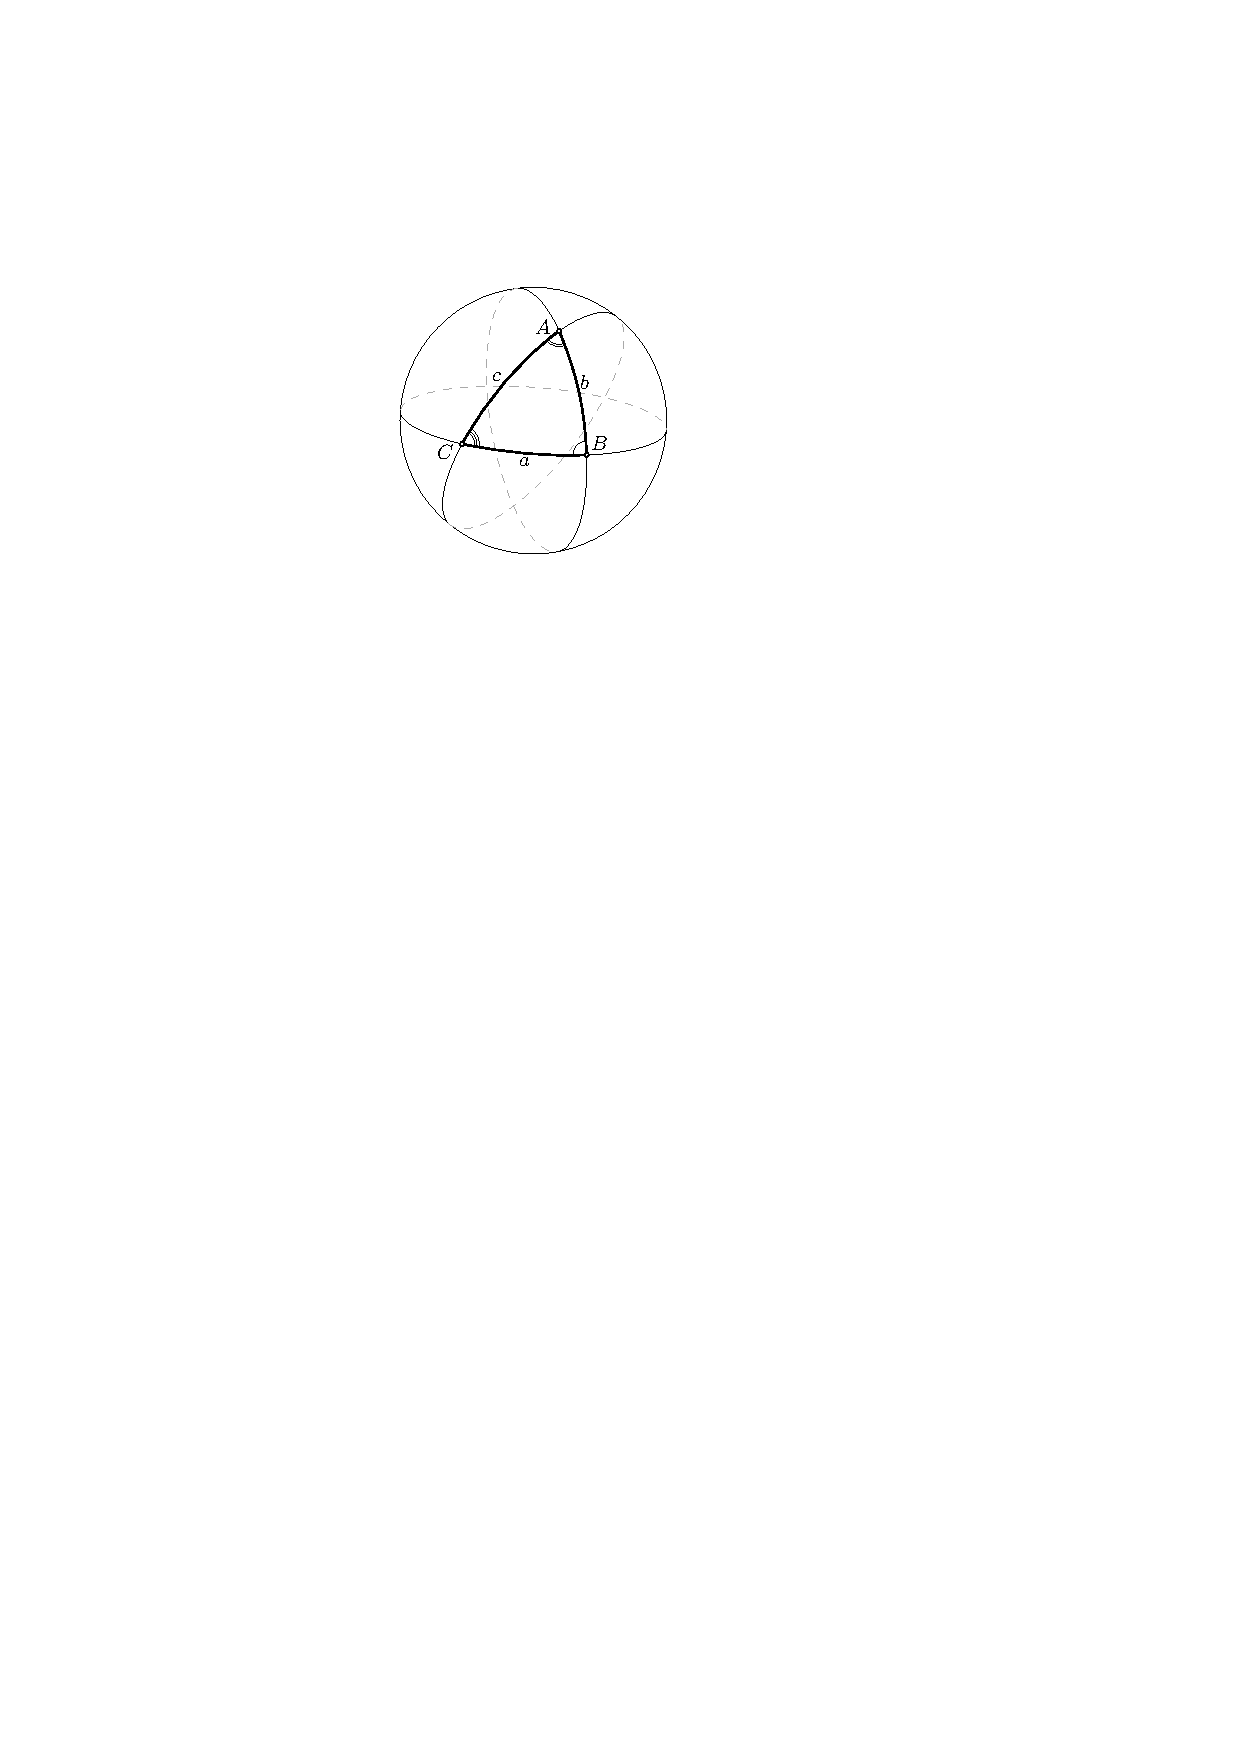
\includegraphics[width=0.4\textwidth]{spher-trigonom}
 \caption{Сферический треугольник}
\end{figure}




